\documentclass[a4paper]{article}

\usepackage[per-mode=symbol,separate-uncertainty=true]{siunitx}
\usepackage{amsmath}
\usepackage{float}
\usepackage{graphicx}
\usepackage[a4paper,top=3cm,bottom=2cm,left=3cm,right=3cm,marginparwidth=1.75cm]{geometry}
\usepackage{mathtools}
\usepackage{siunitx}
\usepackage[colorlinks=true, allcolors=blue]{hyperref}
\usepackage[dvipsnames]{xcolor}

\sisetup{exponent-product=\cdot}

\title{Integrated System Architecture \\ Lab session 3 report - RISC-V special project}
\author{Marco Andorno (247222)\\ Michele Caon (253027) \\ Alessio Colucci (xxxxxx) \\ Matteo Perotti (251453) \\ Giuseppe Sarda (255648)}

\begin{document}
\maketitle

\section{Datapath}
\subsection{Memory}
Both instruction and data memory are implemented using a simple behavioral memory model, with both synchronous read and write operations. According to the specifications of the RV32I, instructions are 32-bit long and the biggest addressable unit is also a 32-bit word, so this data with applies in both cases.

Figure \ref{fig:memory} shows the interface of this block, where the \texttt{address} is left parametric, as it can differ between instructions and data memory. Read and write operations are handled by the couple of control signals \texttt{memRead} and \texttt{memWrite}, of which only one should be asserted at each clock cycle to perform the desired action. Both signals active represent an forbidden condition and should be avoided by the whatever is in charge of controlling the memory.

\begin{figure}[hbtp]
    \centering
    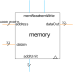
\includegraphics[scale=1]{../memory/ref/schematic/memory.pdf}
    \caption{Memory}
    \label{fig:memory}
\end{figure}

Figure \ref{fig:memory_timing} shows the usual timing diagram of this fully synchronous memory, according to which both reads and writes take place at the next clock cycle after the proper control signals are asserted.

\begin{figure}[hbtp]
    \centering
    \includegraphics[scale=.8]{../memory/ref/timing/memory_timing.pdf}
    \caption{Memory timing diagram}
    \label{fig:memory_timing}
\end{figure}

\subsection{Register file}
The RISC-V register file is composed of 32 registers, each 32-bit wide (for RV32I), called \texttt{x0} to \texttt{x31}, where \texttt{x0} is a special register hardwired to the value 0, which can turn useful for some instructions. Figure \ref{fig:rf} shows the top level diagram of the register file structure.

\begin{figure}[hbtp]
    \centering
    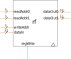
\includegraphics[scale=1]{../register_file/ref/schematic/register_file.pdf}
    \caption{Register file}
    \label{fig:rf}
\end{figure}

Writes to the register file are, of course, synchronous and happen on the positive edge of the clock. For a correct write operation, the destination register must be selected using the \texttt{writeAddr} port, the input data must be placed on the \texttt{dataIn} port and the signal \texttt{regWrite} must be asserted. Internally, the register file will enable only the selected register using a decoder.

Reads are instead combinational and can occur on two different registers at a time, thanks to two different read ports. To select the correct output value, a 32-to-1 multiplexer is used on each read port. However, in order to avoid data hazards during the write back stage, the register file also implements bypassing of input data directly to the output if the same register is read and written during the same clock cycle. Figure \ref{fig:rf_read} shows this read selection process (no multiplexer is used to select 0 in case the register being read is \texttt{x0} as we can suppose it is hardwired directly at its output).

\begin{figure}[hbtp]
    \centering
    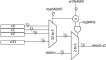
\includegraphics{../register_file/ref/schematic/register_file_deep.pdf}
    \caption{Read operation in the register file}
    \label{fig:rf_read}
\end{figure}

To better illustrate the behavior of the register file operations, their timing diagram is shown in \ref{fig:rf_timing}.

\begin{figure}[hbtp]
    \centering
    \includegraphics[scale=.8]{../register_file/ref/timing/rf_timing.pdf}
    \caption{Register file timing}
    \label{fig:rf_timing}
\end{figure}

\subsection{ALU}

\subsection{Branch and Jump management}
\paragraph{Types of instructions}
There are two classes of instructions which can lead to a modification of the sequential flow of the program. In the RV32I ISA they are:
\begin{enumerate}
	\item Branches
	\item Jumps
\end{enumerate} 
The former is a conditional change of the usual choice of the next address to be put in the PC, whereas the latter is unconditional. The condition, whenever present, is always based on the result of an ALU comparison.

The \textbf{Branch} instruction exists in different flavours, depending upon which comparison has to be performed between the content of two registers. It follows a list of all of them:
\begin{enumerate}
	\item BEQ
	\item BNE
	\item BLT
	\item BGE
	\item BLTU
	\item BGEU
\end{enumerate} 
All these instructions belong to the B type one. They have an immediate field split along the word, which indicates an effective immediate divided by two. Indeed, with a RISC-V standard architecture it is possible to address this way an half of a word at most, but never the single byte.
The effective immediate is calculated with a bit-reorganization, a sign extension and a left shift of one position, to reach the final 32-bits width.
The instruction contains also the addresses of two registers, whose content will be compared by the ALU to decide whether to take the branch or not. 
To distinguish which type of comparison is needed, it is necessary to know the instruction field func3.

The \textbf{Jump} instruction can be of two types, each bringing to a different hardware path for the data:
\begin{enumerate}
	\item JAL
	\item JALR
\end{enumerate}
\textbf{JAL} is a J instruction, whereas \textbf{JALR} is an I one. This difference is reflected on the HW implementation: more on this later.
A jump instruction is unconditional, but still need for an address computation. This operation is different for the two instructions: for JAL it is sufficient to use the branch-addr-computation hardware, whereas JALR requires the non shifted immediate to be added to the content of a register (the next address is not derived by the current one).

\paragraph{Instruction execution}
Since so far no \textbf{BPU} (\textbf{B}ranch \textbf{P}rediction \textbf{U}nit) is present in the design, a "branch not taken" assumption is always done when the content of the PC is updated and the decoded instruction is a \textbf{BR}anch. The simplest way to manage a branch is to delay the decision until the execution stage, waiting for the ALU to do the comparison. The effective decision is then taken in the MEM stage, not to exacerbate a path which can be critical by itself. 
Also the calculation of the next address, which involves the immediate and the program counter, is performed in the execution stage.
A possible improvement could be to anticipate the comparison and the next address calculation in the decoding stage, but to keep the design simple the first solution was chosen.
This is compliant with the calculation of the address for a \textbf{JAL} execution. It is worth to mention that the absence of a condition to be verified is enaugh to simplify the anticipation of the address calculation and bring it in the decode stage. However this solution would increase the number of resources if the other branch/jump instructions are still executed in an another stage.
A \textbf{JALR} instruction beheaves in a slightly different way: the address calculation is performed by the ALU, because the immediate is added to the content of a register.

A branch instruction has no side effects once it has been executed. On the contrary, a jump instruction leaves in the pipeline the next instruction address to be saved in a destination register. This is not a issue though, because it is possible to see that even without forwarding units no data hazards could arise. If the pipline was longer, maybe the forwarding unit would be the only thing to have the day saved (the design has it, though).

\paragraph{Effective calculation}
The address calculation in case of branches/jumps is performed in the execution stage and it depends on the type of instruction:
\subparagraph{Branch/JAL} It is based on the "current" PC value (current for that precise instruction!). The immediate is sign extended, one position left shifted and added to the PC value (percolated through the pipeline until there) by means of another adder. In the meantime, if the instruction is a JAL, the address of the next instruction goes on through the stages.
\subparagraph{JALR} It involves a sum between an immediate and the content of a register. The ALU performs this operation without shifting the immediate. When the result has to be used, the LSB is substituted with a zero. Even in this case, the address of the next instruction follows its path towards the write-back stage.

\paragraph{Next address selection CU}
To control the multiplexers for the next address selection, there's the need for knowing:
\begin{enumerate}
	\item Whether the instruction in the MEM stage is a branch or a jump.
	\item Which is between the two.
	\item The result of the comparison.
	\item If the instruction is a JALR.
\end{enumerate}
The main CU generates two signals \textbf{branch} and \textbf{jump} which percolate along the pipeline, to allow the "Next address selection CU" to solve the first two points. The result of a comparison is simply the LSB of the ALU result. 
The main CU has to generate another signal "jalr" to indicate a JALR instruction.

The "jump" control signal is used also in the writeback stage, to select the right input for the register file. If a jump is performed, the data to be written in the destination register is the "next" address wrt the jump instruction. 

In any case, the IMEM pipe register, together with IF/ID, ID/EX and EX/DMEM ones, have to be flushed. This brings to a performance loss of 4 instructions for each taken branch or executed jump.

\paragraph{Next address generation}
The next address is chosen by means of two multiplexers. The first \textbf{BRJAL\_JALR\_MUX} takes in input the result of the ALU with the LSB masked, and the output of the additional adder of the execution stage. These two input come from the EX/DMEM pipe register. The ouput of \textbf{BRJAL\_JALR\_MUX} is one of the input of the other multiplexer \textbf{NEXT\_PC\_MUX}; the other input is the content of the PC + 4.

\end{document}